\documentclass[12pt]{article}

\usepackage{a4wide}
\usepackage[utf8]{inputenc}

\usepackage{graphicx}
\usepackage{mathtools}
\usepackage{placeins}

\pagestyle{empty}

%\parindent=0pt

\def\mvec#1{\mathbf{#1}}

\begin{document}

\section*{Perspective Transform}

In this exercise, we'll implement a perspective transform to place one image into another one.
The result is shown in Fig. \ref{fig:result}.

A perspective transform is defined by the following equation

\begin{equation}
    \label{eq:proj}
    \begin{bmatrix}
        \phi(x, y) \\
        \psi(x, y) \\
        \omega(x, y)
    \end{bmatrix}
    =
    \begin{bmatrix}
        p_{11} & p_{12} & p_{13} \\
        p_{21} & p_{22} & p_{23} \\
        p_{31} & p_{32} & p_{33}
    \end{bmatrix}
    \begin{bmatrix}
        x \\
        y \\
        1
    \end{bmatrix}
    \, ,
\end{equation}
where homogeneous coordinates after transform are $\phi(x, y)$, $\psi(x, y)$, and $\omega(x, y)$.
The corresponding affine coordinates are then $\phi(x, y) / \omega(x, y)$ and $\psi(x, y) / \omega(x, y)$.

\begin{figure}[th]
    \begin{center}
        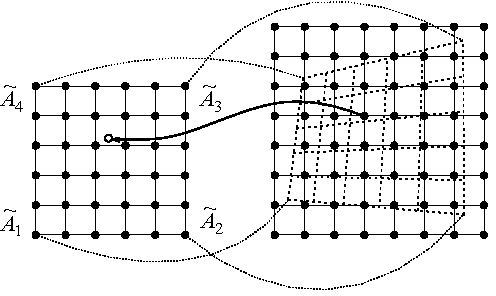
\includegraphics[scale=1.0]{img_6_7}
    \end{center}
    \caption{Projective transform of image.}
    \label{img:6_7}
\end{figure}

Lets consider a projective transform described so that for four points $\tilde{A}_{1} ,\tilde{A}_{2} ,\tilde{A}_{3} ,\tilde{A}_{4}$
in an input image there are corresponding four points $A_{1} ,A_{2}, A_{3}, A_{4}$ defined in an output image
(in Fig. \ref{img:6_7} points $\tilde{A}_{1}, \tilde{A}_{2}, \tilde{A}_{3}, \tilde{A}_{4}$ are chosen as corner points).
Lets illustrate the algorithm to derive the transform matrix from Eq.~\eqref{eq:proj}.
Coordinates of point $\tilde{A}_{i}$ in the input image will be denoted as $\tilde{x}_{i}, \tilde{y}_{i}$.
Location of a corresponding point $A_i$ in the output image is described using $x_i$, $y_i$ coordinates.
Further, lets denote $\mathbf{p}_1 = (p_{11}, p_{12}, p_{13})^\top$, $\mathbf{p}_2 = (p_{21}, p_{22}, p_{23})^\top$, $\mathbf{p}_3 = (p_{31}, p_{32}, p_{33})^\top$, $\mathbf{x}_i = (x_i, y_i, 1)^\top$.
Based on the Eq.~\eqref{eq:proj},for each of the input points we obtain

\begin{equation}
    \label{eq:tri}
\left[\begin{array}{c} {\tilde{w}_{i} \tilde{x}_{i} } \\ {\tilde{w}_{i} \tilde{y}_{i} } \\ {\tilde{w}_{i} } \end{array}\right]=\left[\begin{array}{c} {\mvec{p}_{1}^\top} \\ {\mvec{p}_{2}^\top} \\ {\mvec{p}_{3}^\top} \end{array}\right]\mvec{x}_{i} \, .
\end{equation}
From the third equation in the formula (Eq.~(\ref{eq:tri})) we get $\tilde{w}_{i} = \mathbf{p}_3^\top \mathbf{x}_{i}$.
By substituting it into the first and second equation, we obtain

\begin{equation}
    \label{eq:our_proj}
    \left[
    \begin{array}{ccc}
    \mathbf{x}_i^\top & \mathbf{0} & -\tilde{x}_i \mathbf{x}_i^\top \\
    \mathbf{0} & \mathbf{x}_i^\top & -\tilde{y}_i \mathbf{x}_i^\top
    \end{array}
    \right]
    \left[
    \begin{array}{c}
    \mathbf{p}_1 \\
    \mathbf{p}_2 \\
    \mathbf{p}_3
    \end{array}
    \right]
    =
    \left[
    \begin{array}{c}
    0 \\ 0
    \end{array}
    \right].
\end{equation}

A complete version of Eq.~(\ref{eq:our_proj}) looks as the following

\begin{equation}
    \label{eq:line_extended}
    \begin{bmatrix}
        x_i & y_i & 1 & 0   & 0   & 0 & -\tilde{x}_i x_i & -\tilde{x}_i y_i & -\tilde{x}_i \\
        0   & 0   & 0 & x_i & y_i & 1 & -\tilde{y}_i x_i & -\tilde{y}_i y_i & -\tilde{y}_i
    \end{bmatrix}
    =
    \begin{bmatrix}
        0 \\
        0
    \end{bmatrix}
    \, .
\end{equation}

At this point, we have 8 equations of 9 unknowns.
To solve this issue, we can simply move the first column of the matrix in Eq.~(\ref{eq:line_extended}) to the right side of the equation.
By doing so, we obtain the following system of equations

\begin{equation}
    \label{eq:line_with_right_side}
    \begin{bmatrix}
        y_i & 1 & 0   & 0   & 0 & -\tilde{x}_i x_i & -\tilde{x}_i y_i & -\tilde{x}_i \\
        0   & 0 & x_i & y_i & 1 & -\tilde{y}_i x_i & -\tilde{y}_i y_i & -\tilde{y}_i
    \end{bmatrix}
    =
    \begin{bmatrix}
        -x_i \\
        0
    \end{bmatrix}
    \, .
\end{equation}

We still have 9 unknowns.
The most easiest way to solve this system of equations is to set one of the coefficient of the perspective matrix to a fixed number, for example, $p_{11} = 1.0$
and compute the rest of coefficients using Eq.~(\ref{eq:line_with_right_side}).

\section*{Implementation Details}

To implement the perspective transform, you can use the following coordinates to define the correspondence between each point in the transform (staring from the top left corner in clockwise order):
\\
\\
\noindent
\textbf{Flag}: $(0, 0)$, $(323, 0)$, $(323, 215)$, $(0, 215)$\\
\textbf{Building}: $(69, 107)$, $(227, 76)$, $(228, 122)$, $(66, 134)$
\\
\\
\noindent
To solve system of equations, use OpenCV's \texttt{solve} function.

\newpage

\FloatBarrier
\section*{Expected Output}

\begin{figure}[h]
    \centering
    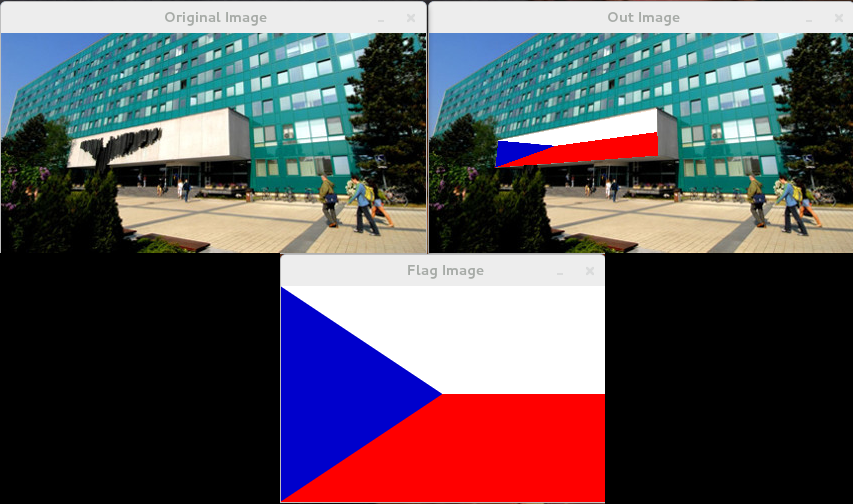
\includegraphics[width=0.8\textwidth]{persp_proj.png}
    \caption{Input image (\textit{top left} and \textit{bottom} images); output image (\textit{top right} image).}
    \label{fig:result}
\end{figure}

\end{document}

